\documentclass[../main.tex]{subfiles}
\graphicspath{
    {"../img/"}
    {"img/"}
}

\begin{document}
\begin{tw}
    Niech $\Omega\subset\mathbb{C}$, $\Omega$ - otwarty i spójny, $A\subset\Omega$. Niech $D\subset A$ - zbiór zer funkcji $f(z)$ na $A$. Niech $P\subset A$ - zbiór biegunów funkcji $f$ na $A$ oraz
    \[
    \partial A \cap \partial D = \phi,\quad \partial A \cap P = \phi
    .\]
Wówczas
\[
    \frac{1}{2\pi i }\int\limits_{\partial A} \frac{f'}{f} = N_Z - N_B
,\]
gdzie $N_Z$ - suma krotności wszystkich zer funkcji $f$ na $A$, a $N_B$ - suma stopni wszystkich biegunów $f$ na $A$.
\end{tw}
\begin{proof}
    Wiemy, że
    \[
        \frac{1}{2\pi i}\int\limits_{\partial A}\frac{f'}{f} = \sum \Res \frac{f'}{f} = \sum_{z_i \in D} \frac{f'}{f} + \sum_{z_k\in P} \frac{f'}{f}
    ,\]
jest sumą krotności wszystkich zer plus sumą krotności wszystkich biegunów, bo jeżeli $z_i\in D$ - zero rzędu $k$, to $\Res \frac{f'}{f} = k$, a jeżeli $z_j\in P$ - biegun rzędu $n$, to
    \[
        \underset{z_j}{\Res}\quad \frac{f'}{f} = -n
    .\]
\end{proof}
\begin{tw}
    (Rouche)\\
    Niech $A\subset\Omega$, $\Omega$ - otwarty i spójny, $f,g$ - holomorficzne na $\Omega$ i taka, że
    \[
        \left| g(z) \right| < \left| f(z) \right|
    ,\]
dla $z\in A$, $f(z) \neq 0$, $z\in \partial A$.
    Wówczas funkcja $f(z) + g(z)$ ma taką samą ilość zer (wraz z krotnościami), co funkcja $f(z)$.
\end{tw}
\begin{proof}
    Niech $a\in \left[ 0,1 \right] $. Rozważmy
    \[
        h_a(z) = f(z) + a\cdot g(z)
    .\]
Wówczas
\[
    N(a) = \frac{1}{2\pi i} \int\limits_{\partial A}\frac{h'_a(z)}{h_a(z)} = \frac{1}{2\pi i}\int\limits_{\partial A} \frac{f'(z) + a g'(z)}{f(z) + ag(z)}
.\]
Zauważmy, że $N(a)$ jest ciągła ze względu na $a$ (jako całka z parametrem). Z drugiej strony,
\[
    N(0) = \frac{1}{2\pi i}\int\limits_{\partial A} \frac{f'(z)}{f(z)} = N_z \text{ funkcji } f
.\]
Skoro wartość $N(0)$ jest liczbą naturalną, a $N(a)$ jest funkcją ciągłą, to znaczy, że $N(0) = N(a) = N(1)$, a
\[
    N(1) = \frac{1}{2\pi i}\int\limits_{\partial A}\frac{f' + g'}{f+g} = N_2 \text{ funkcji }(f+g)
.\]
\end{proof}
\begin{przyklad}
    (Dowód zasadniczego twierdzenia algebry v2.0)\\
    Niech $f(z) = a_0z^n$ i $g(z) = a_1z^{n-1} + a_2z^{n-2} + \ldots + a_{n-1}z + a_n$.\\
    Zauważmy, że
    \[
        \frac{\left| f(z) \right| }{\left| g(z) \right| } \underset{|z|\to \infty}{\longrightarrow} +\infty
    .\]
Możemy zatem wybrać taki zbiór $A$, dla którego $|g(z)| < |f(z)|$, $z\in \partial A$, w którym zawarte będą wszystkie zera funkcji $g(z)$.\\
    Zauważmy, że funkcja $f(z)$ ma zero $n$ - tego stopnia, czyli $N_z = n$ dla funkcji $f$. Oznacza to, że ilość zer wraz z krotnościami (na mocy tw. Rouche) funkcji $f+g$ wynosi $n.\quad \Box$
\end{przyklad}
\begin{przyklad}
    (Sumowanie szeregów v2.0)\\
    \[
    \sum_{n=1}^{\infty} \frac{1}{n^2} = \frac{\pi^2}{6}
    .\]
Ile to będzie \[
\sum_{n=1}^{\infty} \frac{1}{n^4}?
\]
    Niech
    \[
        f(z) = \frac{1}{a^2 - z^2},\quad a\neq \mathbb{Z}
    .\]
Zatem
\[
    \frac{1}{\pi}\sum_{n=-\infty}^{+\infty} f(n) = \underset{z = a}{\Res} \quad \frac{\ctg(\pi z)}{a^2 - z^2} + \underset{z = -a}{\Res} \quad \frac{\ctg(\pi z)}{a^2 -z^2}
.\]
Ale
\[
    \underset{z = a}{\Res} \quad \frac{1}{a^2 - z^2}\ctg(\pi z) = \Res \frac{1}{(a-z)(a+z)} \ctg(\pi z) = \lim\limits_{z\to a} \frac{z-a}{(a-z)(a+z)}\ctg(\pi z) = -\frac{\ctg(\pi a)}{2a}
.\]
Analogicznie $\frac{1}{a^2 - z^2}\ctg(\pi z) = \frac{\ctg(-\pi a)}{2a}$. Zatem
\[
    \sum_{n=-\infty}^{+\infty} \frac{1}{a^2-n^2} = - \frac{\ctg(\pi a)}{a}
.\]
\[
    \sum_{n=-1}^{-\infty} \frac{1}{a^2 - n^2} + \sum_{n=1}^{\infty} \frac{1}{a^2 - n^2} + \frac{1}{a^2} = - \frac{\ctg(\pi a)}{a}
.\]
\begin{equation}
    \label{eqn:w17-1}
    \sum_{n=-1}^{\infty} \frac{a}{a^2 - n^2} + \sum_{n=1}^{\infty} \frac{a}{a^2 - n^2} + \frac{1}{a} = -\ctg(\pi a)\tag{$\star$}
\end{equation}
Ale
\[
    \frac{a}{a^2 - n^2} = \frac{1}{2}\left( \frac{1}{a-n} + \frac{1}{a+n} \right)
.\]
\[
    \sum_{n=1}^{-\infty} \frac{a}{a^2 - n^2} + \sum_{n=1}^{\infty} \frac{a}{a^2 - n^2} = 2 \sum_{n=1}^{\infty} \frac{a}{a^2 - n^2} = \sum_{n=1}^{\infty} \frac{1}{a-n} + \frac{1}{a+n}
.\]
Zatem
\[
    \eqref{eqn:w17-1}:\quad \ldots + \frac{1}{a-n} + \frac{1}{a-(n-1)} + \ldots + \frac{1}{a-1} + \frac{1}{a} + \ldots + \frac{1}{a+n} + \ldots = \ctg(\pi a)
.\]
Wyrażenie po prawej stronie jest funkcją okresu $1$.
\end{przyklad}
\subsection{Residuum w $+\infty$ }
\[
    f(z) = \ldots + \frac{a_{-n}}{z^n} + \frac{a_{-(n-1)}}{z^{n-1}} + \ldots + \frac{a_{-1}}{z^{-1}} + a_0 + a_1 z + \ldots + a_n z^n
.\]
\begin{przyklad}(bijekcja szprychowa - rys \ref{fig:w17-1})
    \begin{enumerate}[i)]
        \item  Chcemy aby $f(x) = \frac{1}{x}$ (na $\mathbb{R}$ ) była ciągła w $x = 0$.
            \[
                \lim\limits_{x\to 0^-}f(x) = -\infty
            ,\]
        \[
            \lim_{x \to 0^+}f(x) = +\infty
        .\]
    \[
        \frac{1-y'}{x'} = \frac{y'}{x - x'} \implies x - x' - xy' + y'x' = y'x' \implies x(1-y') = x'
    .\]
\[
\begin{cases}
    x = \frac{x'}{1-y'}\\ \left(x'\right)^2 + \left(y'\right)^2 = 1
\end{cases}
.\]
Uzwarcenie aleksandrowe $\mathbb{R}\sim 0$, $\overline{\mathbb{R}} \sim 0$ - zamknęliśmy nieskończoności w zerze.
    \end{enumerate}
    \begin{figure}[h]
        \centering
        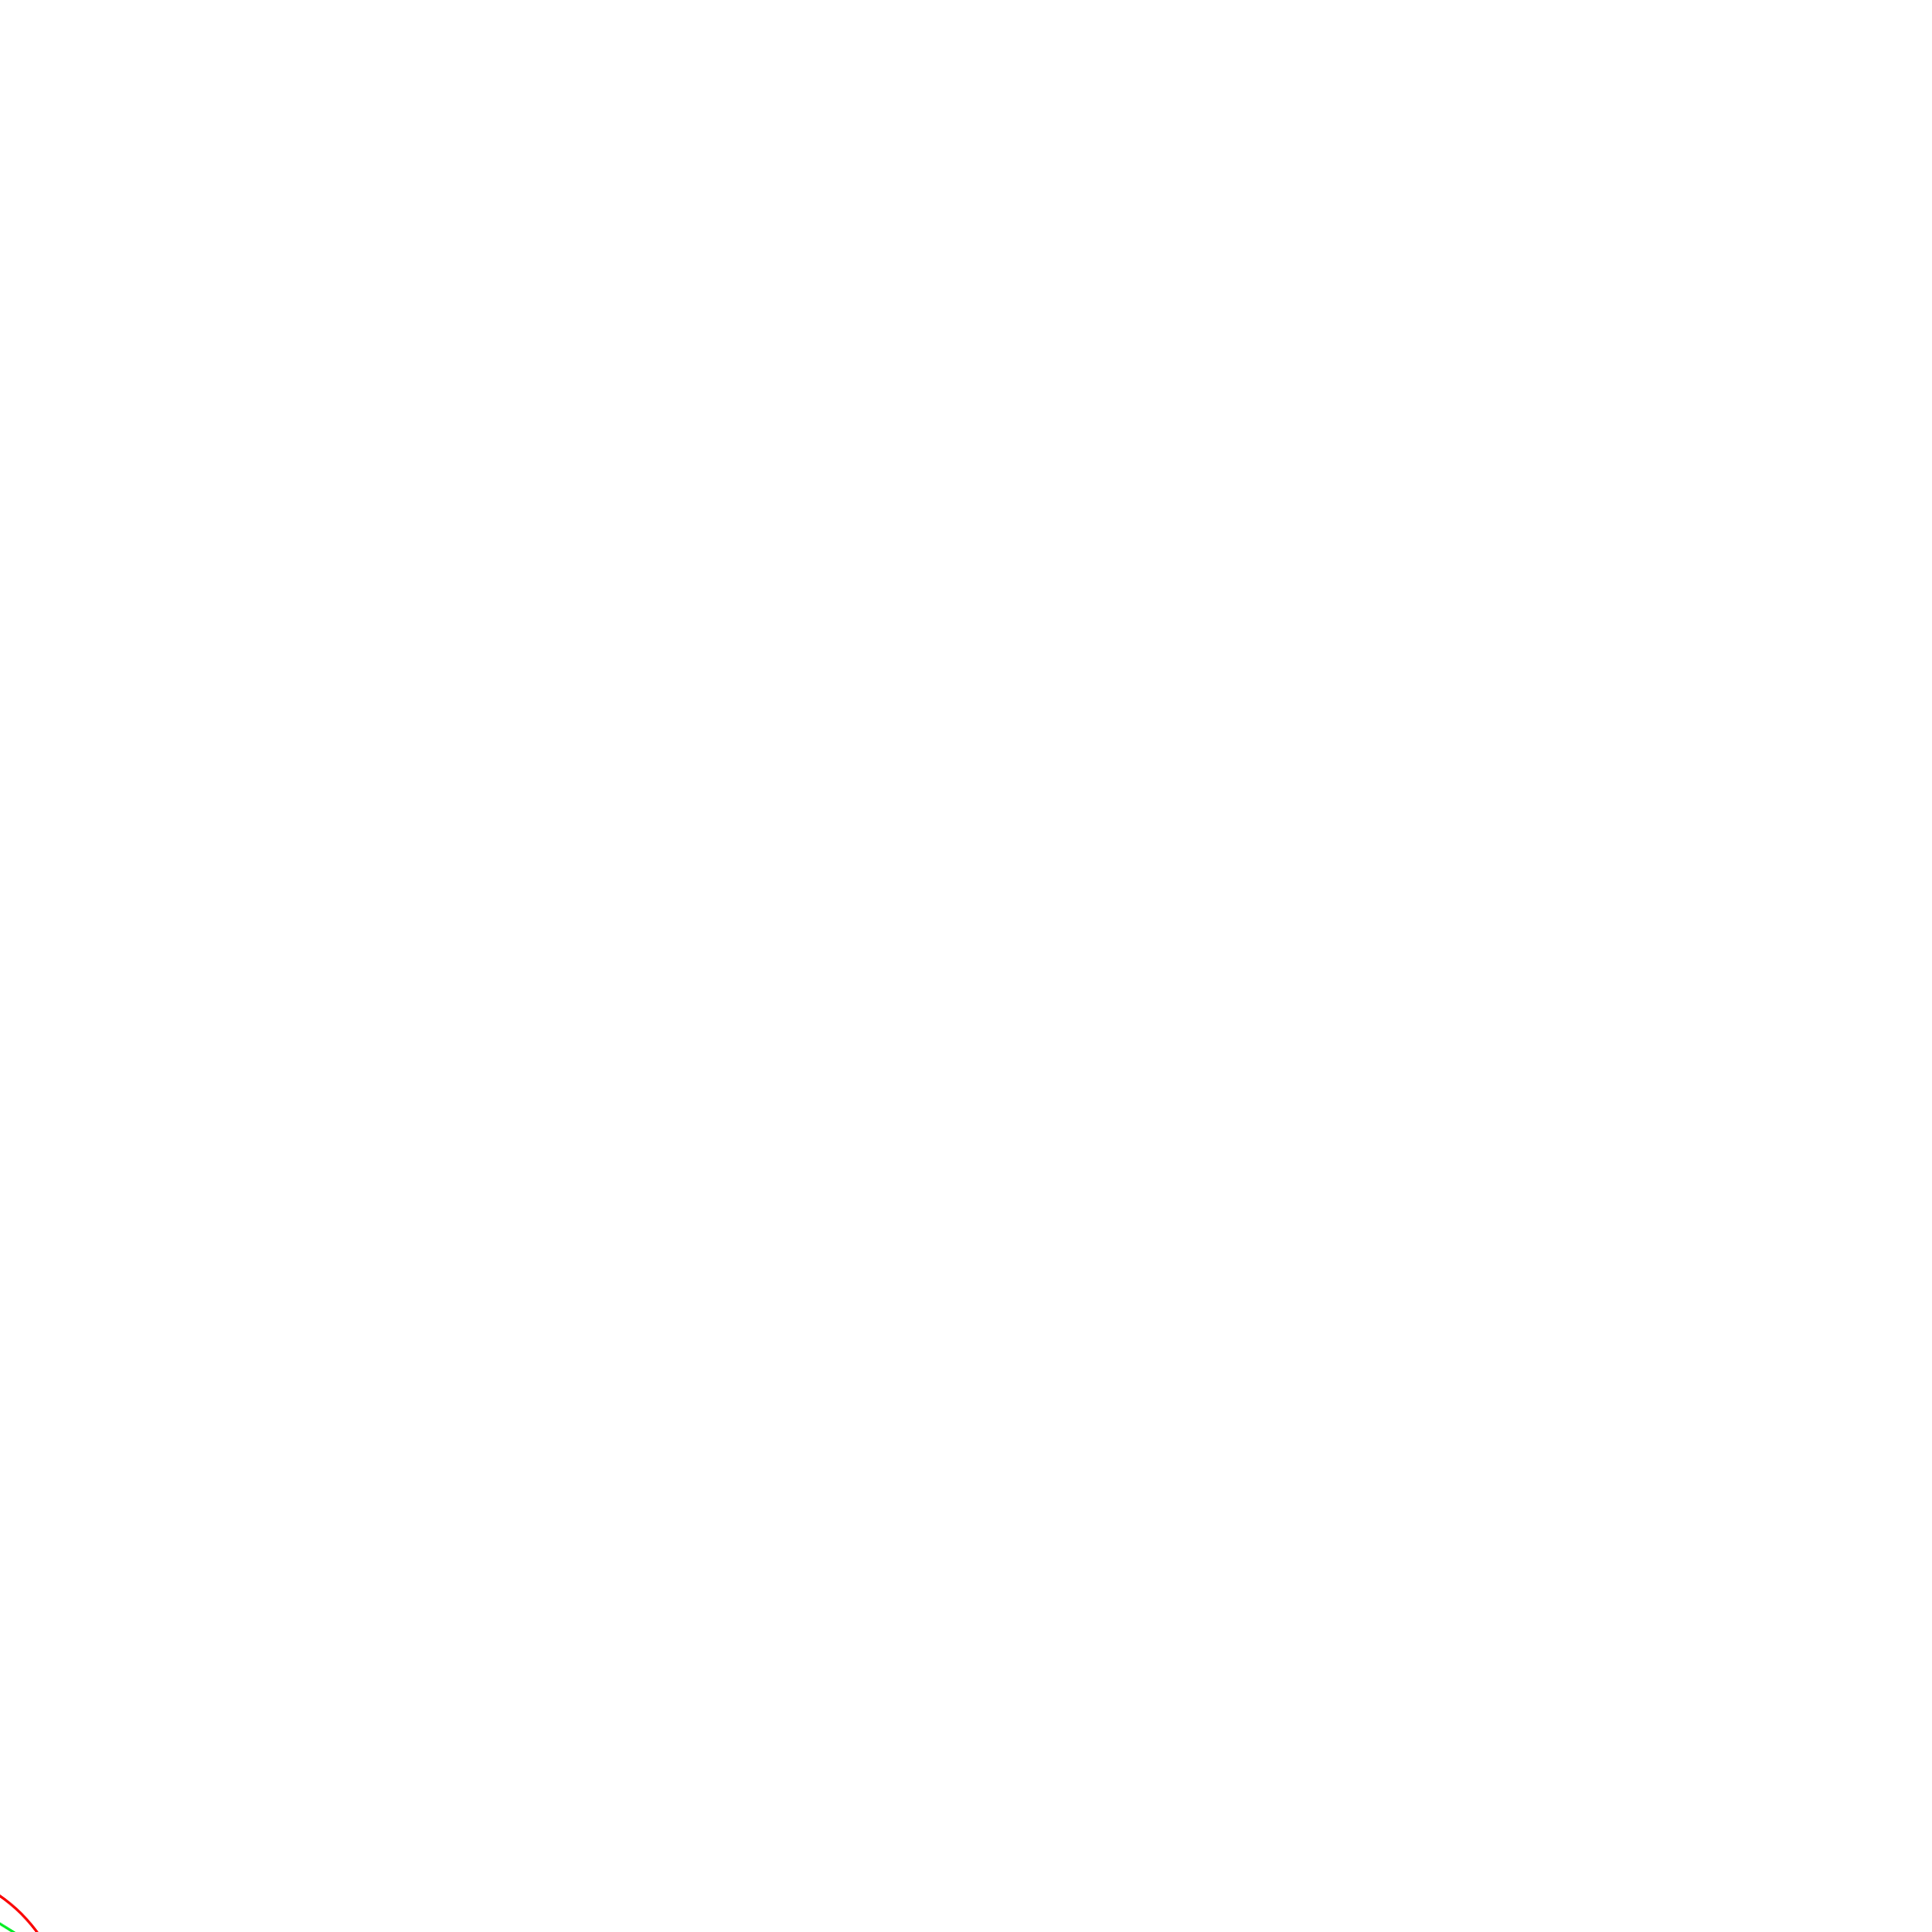
\includegraphics[width=0.45\textwidth]{w17-1}
        \caption{Taka szprycha niech przecina nam okrąg}
        \label{fig:w17-1}
    \end{figure}
\end{przyklad}

\begin{definicja}
    \[
        \overline{\mathbb{C}} = \mathbb{C} + (0,0,1)
    .\]
Mówimy, że $f(z)$ jest holomorficzna w $z = \infty$, jeżeli funkcja $g(z) = f(\frac{1}{z})$ jest holomorficzna w $z = 0$.
 \[
     g(z) = a_0 + a_1(z-z_0) + a_2(z-z_0)^2 + \ldots \quad K(0,R)
.\]
\end{definicja}
\begin{definicja}
Jeżeli  $g(z)$ w rozwinięciu $R(0,0,r)$ ma postać
\[
    g(z) = \frac{a_{-k}}{z^k} + \frac{a_{-(k-1)}}{z^{k-1}} + \ldots + a_0 + a_1z
,\]
to mówimy, że $f(z)$ ma w $z = \infty$ biegun rzedu $k$.
\end{definicja}
\begin{definicja}
    Jeżeli $\lim_{z \to 0}g(z)$ nie istnieje, to mówimy, że $f(z)$ ma w $z = \infty$ osobliwośc istotną.
\end{definicja}
\textbf{Obserwacja:} Jeżeli
\[
    g(z) = \frac{a_{-k}}{z^k} + \frac{a_{-(k-1)}}{z^{k-1}} + \ldots + a_0 + a_1z + a_2z^2 + \ldots
,\]
to
\[
    f(z) = g\left(\frac{1}{z}\right) = a_{-k}z^{k-1} + \ldots + a_0 + \frac{a_1}{z} + \frac{a_2}{z^2} + \ldots
.\]

\end{document}
